\section{Product perspective}
\label{sec:product_perspective}%

\subsection{Scenarios}
\label{subsec:scenarios}%
\paragraph{Scenario 1: Unregistered ST creates an account}
Aldo Pinesco is looking for an internship to get a taste of the working world, so he decides to join S\&C. First, he opens the website and clicks on the Sign-up button, then he inserts his name, surname, nickname, email and password in order to create a new account.

\paragraph{Scenario 2: ST updated their resume}

\paragraph{Scenario 3: CP creates and publishes a new internship}
The Lazzari Company, which is an established company in the Cybersecurity field, wants to offer a professional internship and reach out to as many students as possible. For doing so, they use the S\&C system, so they first define the internship domain by choosing from the several available options, then they define the topics and technologies adopted still using the suggestions offered by the system, and finally they also define the terms of the internship, such as the possibility of being paid or other benefits that a company can offer. Finally, by clicking on the "Publish" button, the internship will be added to the company's showcase, which can be seen from everyone, and also to the system's database, on which the recommendation algorithm works, so that it can immediately start working to find potentially suitable people.

\paragraph{Scenario 4: CP updates or removes an internship}

\paragraph{Scenario 5: ST receives internship recommendations}
The student Riccardo Pianabasso, who has already uploaded his information, has received a notification from the system informing him about a new internship match. After clicking on the message inbox section, he finds a message with all the information about the internship to which he has been matched. Now he has two options, accept or reject the internship. If he refuses, the match is discarded from the system and the company is notified; if he accepts the system will show either that the company has already accepted/rejected the student for the interview or that the company response is pending.

\paragraph{Scenario 6: ST apply for an internship}

\paragraph{Scenario 7: CP reviews applications for an internship}
The fintech company Sossoldi is looking for an intern to join their budget management team. Their ad received several applications via S\&C. Marco Lazzaro, the hiring manager, accesses the "Applications" section, where he reviews the details of each candidate. After going through their CVs and motivational letters, he selects the three best candidates and contacts them.

\paragraph{Scenario 8: CP contacts a student for an internship}

\paragraph{Scenario 9: CP conducts interviews for candidates}
After both parties accept the application, the company begins to construct questionnaires or tasks to be submitted to the applicant, using the help provided by the system. Once this phase is completed, the company sends the material to the students, who can start the assignments. The system then collects the information and sends it to the company, which can decide how to proceed based on its own policies, such as requiring a personal interview, completing other tasks, or accepting the student.

\paragraph{Scenario 10: User makes a complaint}
While working at Pizza Tech, Emily realizes that her task are different from what was written in the internship description. So she logs into the S\&C platform, goes to the internship page and clicks on the button "File a complaint". Emily fills out the form, clearly stating the differences between the job description and the actual tasks assigned. The complaint is automatically forwarded to her university.

\paragraph{Scenario 11: Users provide feedback after an internship}
After completing his internship at BioTech, Lorenzo receives a notification from S\&C asking him to leave feedback about his experience. He fills out a form indicating aspects such as the skills he gained, the support received from the company, and the clarity of objectives. At the same time, his mentor at BioTech fills out a similar form to evaluate Lorenzo, highlighting his problem-solving skills and enthusiasm. Both feedbacks are stored in the system and will be used to improve future matches.

\paragraph{Scenario 12: UV monitors internship progress}

\paragraph{Scenario 13: UV handles complaints}
The university receives a notification from S\&C about a complaint about one of its students. A partner company has reported that a student failed to show up for a scheduled interview. The university reviews the case details, contacts the student for clarification and sends a response to the company with an explanation and an approach to avoid similar issues in the future.

\paragraph{Scenario 14: S\&C notifies Users about a new matching}
Every day, the S\&C system runs its recommendation algorithms to identify matches between students and internships based on their profiles, preferences, and internship criteria. For instance, Chiara Lombardi, a computer science student specializing in artificial intelligence, receives a notification from S\&C about a new internship opportunity at NeuralNet Solutions. The system highlights that this internship involves working on a project with AI-based recommendation systems, which aligns with Chiara's skills and preferences.

Chiara logs into her account, opens the "Notifications" section, and clicks on the recommended internship. She reviews the details and decides whether to express her interest in the position or dismiss the recommendation. Similarly, NeuralNet Solutions is notified about Chiara's profile matching their internship requirements. They can review her CV and decide whether to contact her for further evaluation.

\paragraph{Scenario 15: S\&C updates ST on the progress of their application}
Franco applied for a data science internship offered by HugeData through the S\&C system. A few days later, he receives a notification that his application has been accepted and he is scheduled for an interview. In the notification, he finds the interview details: the date, time, and a link to join. He confirms his availability by clicking "Accept interview".

\newpage

\subsection{Class diagrams}
\label{subsec:class_diagrams}%

\begin{figure}[H]
    \begin{center}
        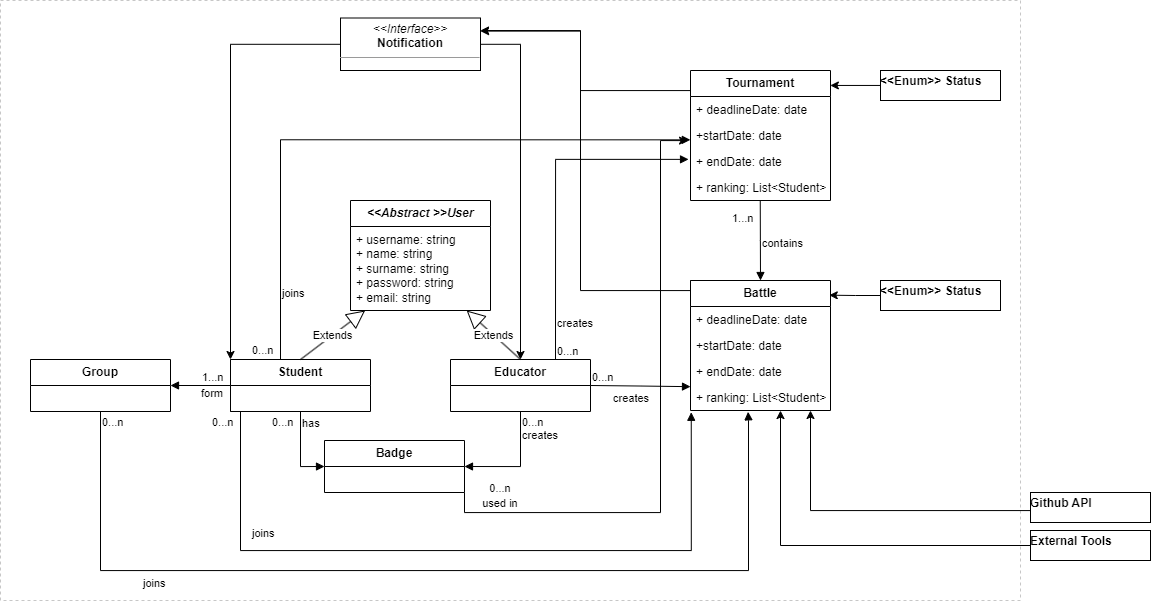
\includegraphics[width=0.9\linewidth]{UML_v2.png}
        \caption{High level Class Diagram.}
        \label{fig:UML}%
    \end{center}
\end{figure}

Student and Educator Classes are implemented by extending the abstract Class ‘User’, since their attributes are almost the same, in fact the Username, name, surname, eMail and password strings are in common for both the classes.\\
EDs may create new instances of the Tournament Class, which contains the Battles. There are two different enumerations (one for Tournament, the other for Battle) in order to implement and to keep record of the current status of the Tournament or the Battle. The current rankings are saved using List<Student> in the correct classes. \\
EDs can also set one or more Badges to be awarded to deserving STs. Battle Class may interact with the external Tools (like the GitHub API and the Tools for the code testing). \\
The Notification Interface is used to send different kinds of notification to STs and EDs when a new Tournament or Battle is created, or during the various phases of the competition, or when a ST invites other STs to join a STG.\\


\subsection{State diagrams}
\label{subsec:state_diagrams}%
In this section are presented the State Diagrams of the CKB system representing all the possibile operation that a User can perform.
\paragraph{Signup.}
When a User wishes to register on CKB, they are required to input their credentials, including their name, surname, nickname, eMail and password in a registration form. If the provided credentials are deemed valid (ensuring that the eMail or nickname is not already in use, and the password meets the criteria of being at least 8 characters long, containing at least one capital letter, a number, and a special character), CKB will send an eMail to the User. Upon the User confirming the registration through the provided eMail link, the new account is successfully created. If the credentials are not correct CKB shows an error message to the User and redirects him to the signup form page.

Furthermore, if the User selects the option "Register as a new Educator" during the registration process, CKB will enhance the account with additional permissions. These permissions may include the possibility to create Tournaments or Battles.

\begin{figure}[H]
    \begin{center}
        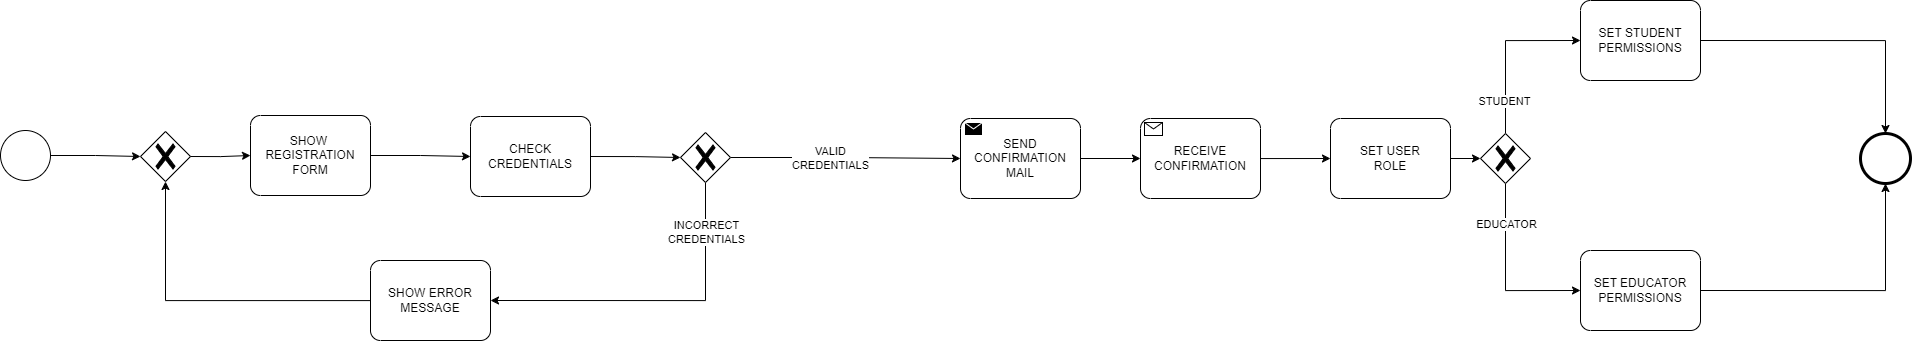
\includegraphics[width=1\linewidth]{StateDiagrams/signup.png}
        \caption{Signup state diagram.}
        \label{fig:signup_sd}%
    \end{center}
\end{figure}

\paragraph{Login.}
When a registered User attempts to log in to their CKB account, they must enter their credentials (eMail and password) into a login form. If the provided credentials are accurate —matching those of a registered User in the CKB database— CKB displays the User's homepage, showcasing Tournaments and ongoing Battles in which the User is participating. On the other hand, if the entered credentials are invalid, CKB presents an error message to the User and redirects them back to the login form page.

\begin{figure}[H]
    \begin{center}
        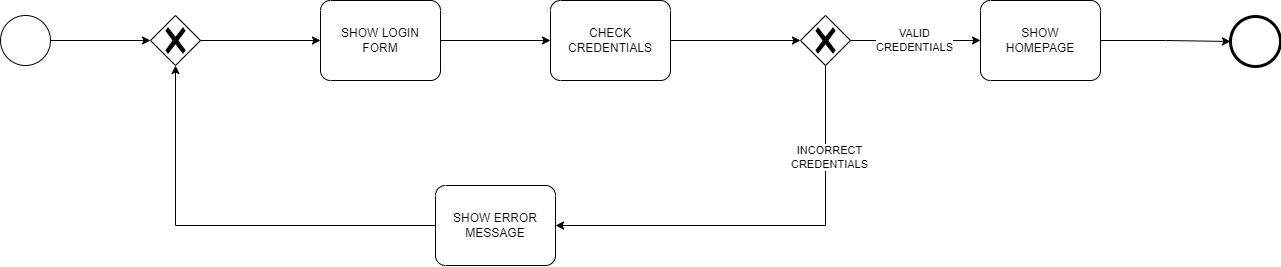
\includegraphics[width=1\linewidth]{StateDiagrams/login.png}
        \caption{Login state diagram.}
        \label{fig:login_sd}%
    \end{center}
\end{figure}

\newpage

\paragraph{Create a Tournament.}
When an ED intends to create a new Tournament on CKB, he is required to input various parameters in the create Tournament form. These parameters include the Tournament name, the registration deadline for the STs and the rules to acquire the Badges. In addition to these parameters, the ED can invite other EDs to join this Tournament, through a notification sent by CKB, to help him create new Battles. If any of these parameters are deemed unacceptable by the system, CKB displays an error message to the ED and redirects him back to the create Tournament form page.

Conversely, if all parameters meet the system's criteria, CKB proceeds to create the Tournament. The newly created Tournament is then added to the ED's Tournaments list, and a notification is sent to all STs to inform them of the availability of a new Tournament.

\begin{figure}[H]
    \begin{center}
        \includegraphics[width=1\linewidth]{StateDiagrams/create Tournament.png}
        \caption{Create a Tournament state diagram.}
        \label{fig:create_Tournament_sd}%
    \end{center}
\end{figure}

\paragraph{Create a Battle.}
Once a Tournament is created, an ED has the option to create a new Battle within it. To do so, the ED is required to input various parameters in the create Battle form. These parameters encompass the Battle name, code kata, registration deadline, submission deadline, minimum and maximum members per STG, and any additional rules for evaluation. In the event that any of these parameters are considered unacceptable by the system, CKB displays an error message to the ED and redirects them back to the create Tournament form page.

Conversely, if all parameters meet the system's criteria, CKB proceeds to create the Battle. The newly created Battle is then added to the ED's list of Battles, and a notification is sent to all STs registered to the Tournament where the Battle resides, informing them that a new Battle is now available.

\begin{figure}[H]
    \begin{center}
        \includegraphics[width=1\linewidth]{StateDiagrams/create Battle.png}
        \caption{Create a Battle state diagram.}
        \label{fig:create_Battle_sd}%
    \end{center}
\end{figure}

\paragraph{Join a Tournament.}
When a new Tournament is created, a ST receives a notification or discovers it on the homepage. At this point, the ST can choose to join the Tournament. If the ST is not yet registered for that specific Tournament, CKB not only adds the Tournament to the ST's Tournament list but also includes the ST in the participant list of the newly created Tournament. This ensures that the ST is officially registered as a participant, allowing him to engage in the Battles.

\begin{figure}[H]
    \begin{center}
        \includegraphics[width=1\linewidth]{StateDiagrams/join Tournament.png}
        \caption{Join a Tournament state diagram.}
        \label{fig:join_Tournament_sd}%
    \end{center}
\end{figure}

\paragraph{Join a Battle.}
Once a ST has registered for a Tournament, and a new Battle is created within it, the ST has the option to join a specific Battle. CKB performs a check to verify if the registration deadline for the chosen Battle has not expired. If the ST is within the allowed timeframe, CKB adds the ST to the list of participants for that Battle and directs them to the create group page where they can further engage in the competition.

However, if the registration deadline has already expired, CKB displays an error message to the ST, notifying them of the expiration, and redirects them to the Tournament dashboard with the respective Battle. This ensures that participants are aware of the registration timeline and can take timely actions to join the Battles of their choice.

\begin{figure}[H]
    \begin{center}
        \includegraphics[width=1\linewidth]{StateDiagrams/join Battle.png}
        \caption{Join a Battle state diagram.}
        \label{fig:join_Battle_sd}%
    \end{center}
\end{figure}

\paragraph{Create a Group.}
The possibility to create a group within a Battle is granted to STs once they have joined a Battle, and the registration deadline has expired. At this point, they are redirected to the create group form, where they write de STG name and can invite other STs to join their STG. The process involves the ST entering a nickname, and upon verification by CKB that the ST with that nickname has also joined the same Battle, a notification is sent to the invited ST, enabling them to join the STG.

Upon receiving a notification, a ST has the option to respond, and upon acceptance, the ST is added to the STG, becoming a participant in the Battle. This invitation process is replicated for each ST that the group creator wishes to invite. Once the group is formed, the ST who initiated the STG can confirm the group, but only if the minimum and maximum number of group members are adhered to. Once confirmed, the STG is ready to actively participate in the Battle.

However, if an invited ST is not part of the Battle, a ST accepts the invitation after the deadline, or the group creation deadline has expired, CKB displays an error message to the respective ST, informing them of the issue and guiding them accordingly. This ensures that the group creation and participation adhere to the specified deadlines and criteria.

\begin{figure}[H]
    \begin{center}
        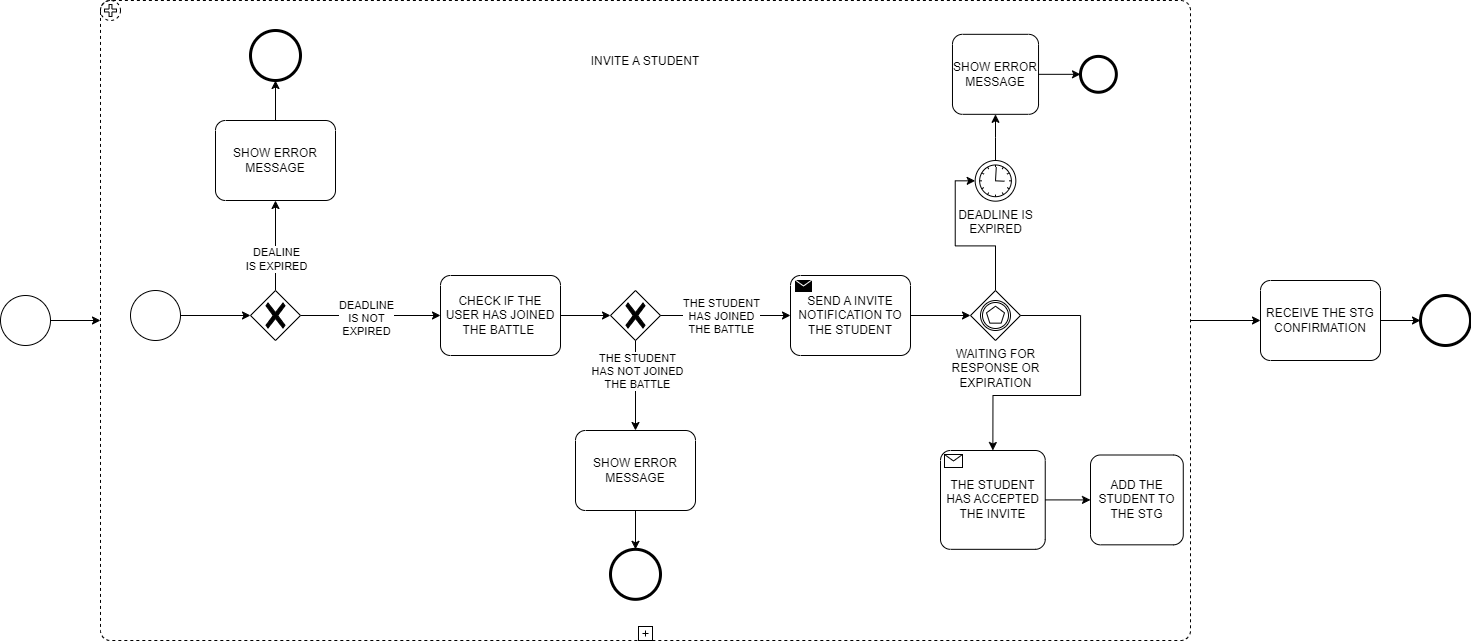
\includegraphics[width=1\linewidth]{StateDiagrams/create group.png}
        \caption{Create a Group state diagram.}
        \label{fig:create_group_sd}%
    \end{center}
\end{figure}

\paragraph{Evaluate the code.}
During the consolidation stage, once all commits have been completed and no further changes are possible, an ED has the option to manually inspect a STG code. The ED can download the code from the Battle dashboard for thorough examination. After reviewing the code, the ED can then modify the score assigned to the STG, which was previously assessed by external tools automatically during each commit.

To facilitate this, CKB provides a form that allows the ED to input the adjusted score. However, before updating the score, CKB checks whether the new score adheres to predefined boundaries, such as being non-negative or not exceeding 100. If the new score meets these criteria, CKB successfully updates the score for the STG.

In the event that the new score falls outside the specified boundaries, CKB displays an error message to the ED and redirects them to the evaluate code form.

\begin{figure}[H]
    \begin{center}
        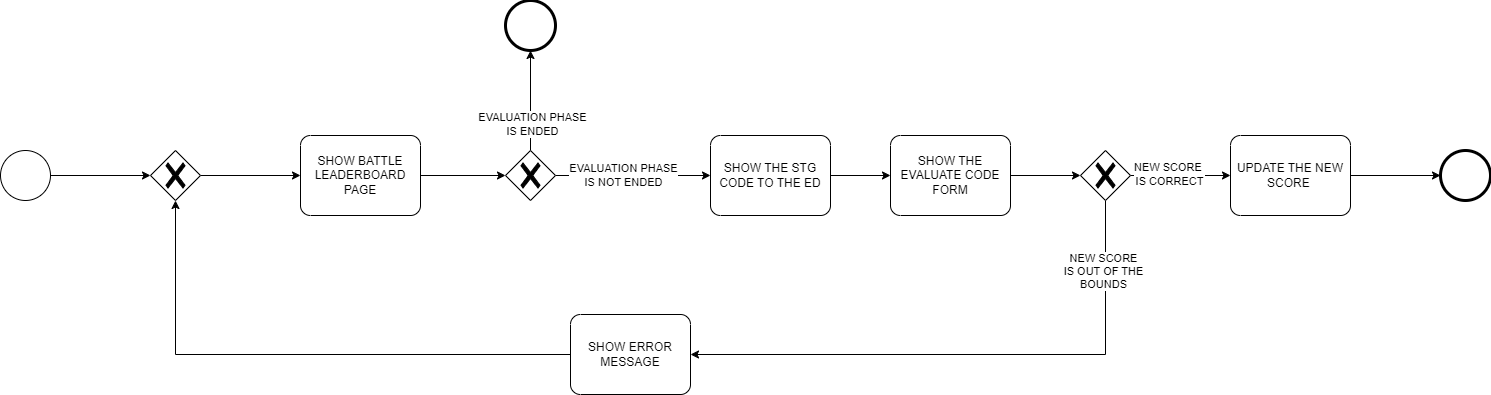
\includegraphics[width=1\linewidth]{StateDiagrams/evaluate code.png}
        \caption{Evaluate the code state diagram.}
        \label{fig:evaluate_code_sd}%
    \end{center}
\end{figure}

\paragraph{Open a profile.}
If a User wishes to view another User's profile, including Badges and other relevant information, they can do so by clicking on the User's nickname in various dashboards, such as the Tournament dashboard or the group composition. Upon clicking the nickname, CKB displays the profile of the selected User to provide the desired information. This feature allows Users to easily access and view the profiles of others within the platform.

\begin{figure}[H]
    \begin{center}
        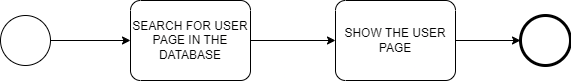
\includegraphics[width=1\linewidth]{StateDiagrams/open a profile.png}
        \caption{Open a profile state diagram.}
        \label{fig:open_profile_sd}%
    \end{center}
\end{figure}

\paragraph{Search for a profile.}
In addition to opening a User profile by clicking the nickname in a dashboard, Users also have the option to use the search bar. By entering a nickname or a keyword in the search bar, CKB will display a list of Users whose nickname contain the entered keyword. Users can then click on a specific User from the search results to open and view their profile, providing a convenient and flexible way to access User information within the platform.

\begin{figure}[H]
    \begin{center}
        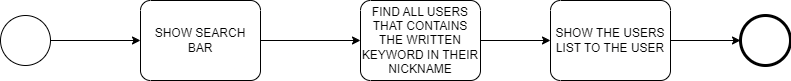
\includegraphics[width=1\linewidth]{StateDiagrams/search for a profile.png}
        \caption{Search for a profile state diagram.}
        \label{fig:search_profile_sd}%
    \end{center}
\end{figure}

\paragraph{Search for a Tournament.}
Users can utilize the search bar to look for Tournaments by entering a name or a keyword. When a search query is entered, CKB will present a list of Tournaments whose names contain the specified keyword. Users can then click on a particular Tournament from the search results, and CKB will redirect them to the Tournament dashboard for detailed information and engagement with the selected Tournament. 

\begin{figure}[H]
    \begin{center}
        \includegraphics[width=1\linewidth]{StateDiagrams/search for a Tournament.png}
        \caption{Search for a Tournament state diagram.}
        \label{fig:search_Tournament_sd}%
    \end{center}
\end{figure}

\paragraph{Logout.}
Users can log out from their account at any time by clicking the "Logout" button. Upon clicking the button, CKB terminates the User's session, ensuring that they are securely logged out. Following this action, the User is then redirected to the login page, providing them with the opportunity to rejoin the CKB system if they wish to do so. 

\begin{figure}[H]
    \begin{center}
        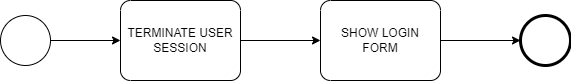
\includegraphics[width=1\linewidth]{StateDiagrams/logout.png}
        \caption{Logout state diagram.}
        \label{fig:logout_sd}%
    \end{center}
\end{figure}

\section{Product functions}
\label{sec:product_functions}%
Here are listed a summary of the main functions of the CKB system:\\\\
\textbf{ Signup:} The User submits his name, surname, nickname, eMail address and a new password. A confirmation mail is required to complete the process.\\\\
\textbf{ Login:}The User sign in after typing his eMail and password in the login form. \\\\  
\textbf{ Create a Tournament:} The ED creates a new Tournament and the system sends a notification to all the STs.\\\\
\textbf{ Join a Tournament:} A ST can join a Tournament by clicking on the “Join Tournament” button on the Tournament’s page.\\\\
\textbf{ Create a Battle:} An ED can create multiple Battles within a Tournament to test the STs. When a new Battle is created CKB sends a notification to all the STs that have joined the Tournament.\\\\
\textbf{ Join a Battle:} A ST can join a Battle by clicking on the “Join Battle” button on the Battle’s page.\\\\
\textbf{ Create a Group:} After joining a Battle the ST may create a new group and invite other STs or accept an invitation to join another STG. It is a choice of the ST to play alone or to create a group with STs, whether this is made possible by the minimum number of STs per STG decided by the ED.\\\\
\textbf{ Evaluate Code:} During the Consolidation phase, an ED can manually download and evaluate the code of a STG within a Battle.\\\\
\textbf{ Create a Badge:} An ED can create Badges to be awarded to worthy STs and define their rules.\\\\
\textbf{ Search for a Profile:} Users can write a nickname or a keyword in the search bar to retrieve another User’s profile.\\\\
\textbf{ Open a Profile:} Users can click on a nickname in a Leaderboard to open another User’s profile.\\\\
\textbf{ Search for a Tournament:} Users can write a Tournament's name or a keyword in the search bar to retrieve the information about a Tournament.\\\\
\textbf{ Logout:} A User session will be closed if the User clicks on "Logout" button. Next time the User opens CKB he will need to log in again.


\section{User characteristic}
\label{sec:User_characteristic}%
There are two types of registered Users in CKB: Students (STs) and Educators (EDs). Here are briefly explained their main characteristics:
\begin{itemize}
    \item ST: Students join CodeKataBattle in order to prove and improve their skills in coding. They need to have a device with an internet connection and an account in order to have access to CKB, in which they can join Tournaments and Battles to compete with other STs.  
    \item ED: Educators join CodeKataBattle, where they can create Tournaments in which STs can compete in different Battles and evaluate the STs’ works.
\end{itemize}
Both the EDs and the STs need to register an account in order to access CKB. During the registration process their both asked to provide an eMail account.

\section{Assumptions, dependencies and constraints}
\label{sec:assumptions_dependencies_constraints}%

\subsection{Domain assumptions}
\label{subsec:domain_assumptions}%
\newcounter{da}
\setcounter{da}{1}
\newcommand{\cda}{\theda\stepcounter{da}}
\begin{center}
    \begin{longtable}{ |l|p{0.9\linewidth}| }
        \hline
        \textbf{ID} & \textbf{Description} \\
        \hline
        DA\cda      & The EDs need to have a valid eMail address. \\
        \hline
        DA\cda      & The STs need to have a valid eMail address. \\
        \hline
        DA\cda      & The EDs need to have a device and a reliable internet connection. \\
        \hline
        DA\cda      & The STs need to have a device and a reliable internet connection. \\
        \hline
        DA\cda      & The EDs need to have a GitHub account. \\
        \hline
        DA\cda      & The STs need to have a GitHub account. \\
        \hline
        DA\cda      & STs need to know how to fork a GitHub Repository. \\
        \hline
        DA\cda      & STs need to know how to push their code on GitHub. \\
        \hline
        DA\cda      & CKB needs to communicate with GH through its API. \\
        \hline
        DA\cda      & CKB needs to communicate with the external Static Analysis Tools in order to compute the scores. \\
        \hline
        DA\cda      & CKB needs to communicate correctly with the eMail system. \\
        \hline
        \caption{Domain assumptions.}
        \label{tab:domainassmptn_tab}%
    \end{longtable}
\end{center}